\section{Introduction}

\comment{ Moved some of the content from the abstract here}
The new milleneum saw an explosion in the developement of such devices and a moving away of users from single computers towards personal computing \cite{Lyle2013}. Now, in 2017, it is commonplace for an average user to own and actively use several computing devices. With new trends and technology comes new challenges and a challenge in security arises when the user needs to manage their multiple interconnected devices and their multiple identities for their applications. The device owner usually relies on some ``Keychain'' app to share the user's cryptographic private key and this key sharing can often be insecure and expose the user to grave security concerns of theft and malware\cite{Atwater2016}. Devices such as phones and watches are frequently removed or replaced. Also, the loss of a single device can compromise the security of the user and their remaining devices.

In the next section, we look at the definition of this problem and look at the various possible solutions that try to solve it.

\section{Background Information}
In section 2.1 we talk about the multi-device problem and describe it. Section 2.2 enumerates the various possible solutions and briefly describes each one.

\subsection{The Multi-device Problem}
The multi-device problem as introduced above is a situation that arises when a user possesses several computing devices at a time. Cryptographic keys that were once simply stored on a single computer are now required by several devices and must somehow be securely distributed across these devices. Users need these to consistently authenticate themselves as single identity across multiple devices. This means that secret keys which are intended to be stored securely are now going to be moved around exposing them to multiple threats of theft such as phishing, pulling them from memory or password cracking attempts (if they are password protected) \cite{Atwater2016}.\\
The simplest solutions to this problem involve either attempting to securely synchronize a single key across multiple devices or to have a per-device key system. While these simple solutions solve the \emph{multi}-device problem, they create a set of new problems that must be addressed\cite{Atwater2016}.

\subsection{Overview of Various Solutions}
We will now present and overview of the several solutions that are capable of resolving the multi-device problem as well as accompanying issues. They are as follows \cite{Atwater2016}:

\begin{itemize}

	\item \textbf{Per-device keys} As described above, the user has an independant key on each device. The idea of per-device keys does not 				really solve the multi-device problem in that the user must generate and maintain several individual keys which is cumbersome. Also, all third 			parties must be made aware of every idividual private key owned by the user to be able to consistently authenticate that user with the same 			identity. Also, unique keys for each device will keep the verifying third party informed of which device the user is currently using. This creates a 	privacy issue where third parties can monitor the usage of a user's devices just from the keys.\\

	\item \textbf{Key sync} This involes the user making several copies of the same secret key and copying them to all devices. This procedure 			has several issues. The act of copying the secret key itself is susceptible to various attacks leading to the key being compromised. If the user 		loses one device than they must update the key for all other devices. This is because the lost device may be used to obtain the secret key and 		compromise all the other devices owned by the user.\\

	\item \textbf{Manual thresholding} The user has per-device keys but embeds and additional police in each signature that tells the verifying 				third party to look for other signatures from other devices belonging to the user. The issue with manual thresholding is the similar to that of 			the simple per-device keys method. A verifying third party can monitor the usage of the user's devices.\\

	\item \textbf{Personal PKI} Is one of the approaches that has seen significant interest and development. It built on the idea of the key sync 			but the user has an additional ``master'' key on one device, or a ``master'' device, or an application whose job it is to validate the other keys 		or devices. It is based on the idea of a public key infrastructure, but in this case it is entirely personal and provides the user with the 						ability to manage their own keys. \comment{[Revise/Add 	more Information]} The obvious disadvantage is that the user has to manage an 				additional ``master'' device/application and that it introduces a simgple point of failure that can be quite disastrous.\\

	\item \textbf{Group Signatures} Group Signatures work on the idea that a single member in the group can sign a message for the other 					members. They present a single key to the third party but internally have separate keys\cite{Bellare2003}. The idea of group signatures can be 	extended to devices where the user uses one device to sign for all the other devices. This idea has been explored for the case of multiple 				password management in the form of Pico\cite{Stajano2011} where the user can use a single device to replace all their PINs and passwords. 			This has not seen significant development for the multiple devices. \\

	\item \textbf{Threshold Cryptography} Is another approach that has seen significant interest and development. It is by far the most promising 		approach as it deals with the multi-device problem and also provides security against lost or theft of a device\cite{Desmedt2001}. In this 				method either the key itself or some cryptographic operations are distributed among the user's $n$ devices\cite{Desmedt1994}. Whenever a 		devices requires to perform a cryptographic operation, either a user defined \emph{threshold} number of devices $t$( where $t \leqslant n$) 		work together to recover the original key or the cryptographic operation itself is distributed over $t$ devices. Any less then t devices will not 		be able to divulge any valuable information.

\end{itemize}

\comment{Add Figure from Shatter showing comparison}

\comment{Add definitions for properties of the schemes}

\section{The \emph{Personal} Key Infrastructure}

The \textit{Personal} Key Infrastructure as a solution to the multi-device problem has seen a fair share of interest over the last decade. The idea of a personal PKI has been around since the last decade. Sinclair et al. wrote their paper during the advent of the smartphone era. It was a time when the multi-device problem was just coming into existence. To cope with it, they developed a solution in the form of \textit{porKI} \cite{Sinclair2005}.

The multi-device problem matured over the years and so did the solutions to combat it. In 2013, Lyle et al. developed and presented \textit{webinos} a cross platform runtime environment that implemented a personal PKI \cite{Lyle2013}. And in 2015, Melara et al. presented CONIKS \comment{a few words about it} \cite{Melara2015}.

Lyle et al.\cite{Lyle2013} outlined a set principles that should be adhered to while developing personal key infrastructures:
\begin{itemize}

	\item \textbf{Leverage existing identities}. Leverage the existing identities that people already have, such as social network accounts, email 			accounts and homepages, and reuse these in public key infrastructures. The authors suggest using a mapping of a social network identity to a 		public key or certificate so that users can find each other using a web-based identitiy.

	\item \textbf{Assume devices are mobile}. Devices such as smartphones, smartwatches, tablets, laptops and cars are all designed to be 					mobile. This makes them prone to being lost or stolen. It is important that the personal PKI implementation take this into account and provide 		for such devices to be removed from the network and their keys revoked.
	
	\item \textbf{Avoid using PKI metaphors}. Users should not be exptected to be familiar with PKI jargon and terminology. They should never be 		asked to make a decision about keys and certificates. All these should happen behind-the-scenes automatically.
	
	\item \textbf{Use web technologies to make networks interoperable}. The authors suggest harnessing the power of web applications to make 		personal networks work for devices that are made to be mobile. A web server can be used to make the personal network available to any 				device that is capable of making outgoing connections.
	
	\item \textbf{Delegate key storage to operating systems}. The authors suggest that key storage should be delegated to the operating 					systems of the specific devices. In the authors' opinion many devices already have secure means of protecting keys such as secure hardware. 			Also, a devices like a smartphone would not have as much authentication requirements as a personal computer. Thus, the problem of key 				storage is best solved in a device-specific manner.
	
	\item \textbf{Device keys are not always a factor of user authentication}. The authors make room for users with shared devices. They suggest 	that device keys should be used only to authentiacte the device and not the user. A device should authenticate just the device. The second 			factor (i.e. authenticating the user) is only appropriate when it is known that the device is single user specific, such as a mobile phone or a 				laptop.
\end{itemize}

\subsection{PorKI}
\comment{Drop old and outdated tech?}

\subsection{\emph{webinos}: Personal PKI for Smart Devices}

\textit{webinos} is an application platform designed and implemented by Lyle et al. \cite{Lyle2013}. It implements a personal network that the authors refer to as a \textit{personal zone}. These so-called personal zones define the devices that are used by a particular person. The personal zone has a master device called a personal zone hub which acts as a certificate authority and can be implemented as an online web service.

\textit{webinos} was developed in 2013 as a cross-platform runtime environment for web applications. It provides a set of JavaScript APIs for webapplications to access local device functionality. For example, a web application could be made to access the camera or the address book of a smartphone. It also provides access control features to restrict and control access using the APIs for the sake of privacy and security.

The architecture of \textit{webinos} and it's implementation of a personal PKI are summarized in the following points:

\begin{enumerate}[label=\arabic*., wide, labelwidth=!, labelindent=0pt]
	\item \textbf{Components and communication} \textit{webinos} consists of the following three componenets spread over various devices:
	\begin{itemize}
			\item Personal Zone Proxy (PZP) This runs on each device and implements the API. It is responsible for communicating with other PZPs, 					the PZH and WRTs. It also performs policy enforcement. PZPs communicate with each other and the PZH over mutually-authnticated TLS 					sessions.
			\item Personal Zone Hub (PZH) The PZH is web-based and constantly available. It routes messages between PZPs and synchronizes access 				control settings. It acts as a certificate authority and issues certificates to the PZPs.
			\item Web Runtime (WRT) Web runtime is used to execute and display web applications. It is the user inferface to web applications
	\end{itemize}

	\item \textbf{Certificate hierarchy}
		\begin{figure*}[!h]
			\centering
			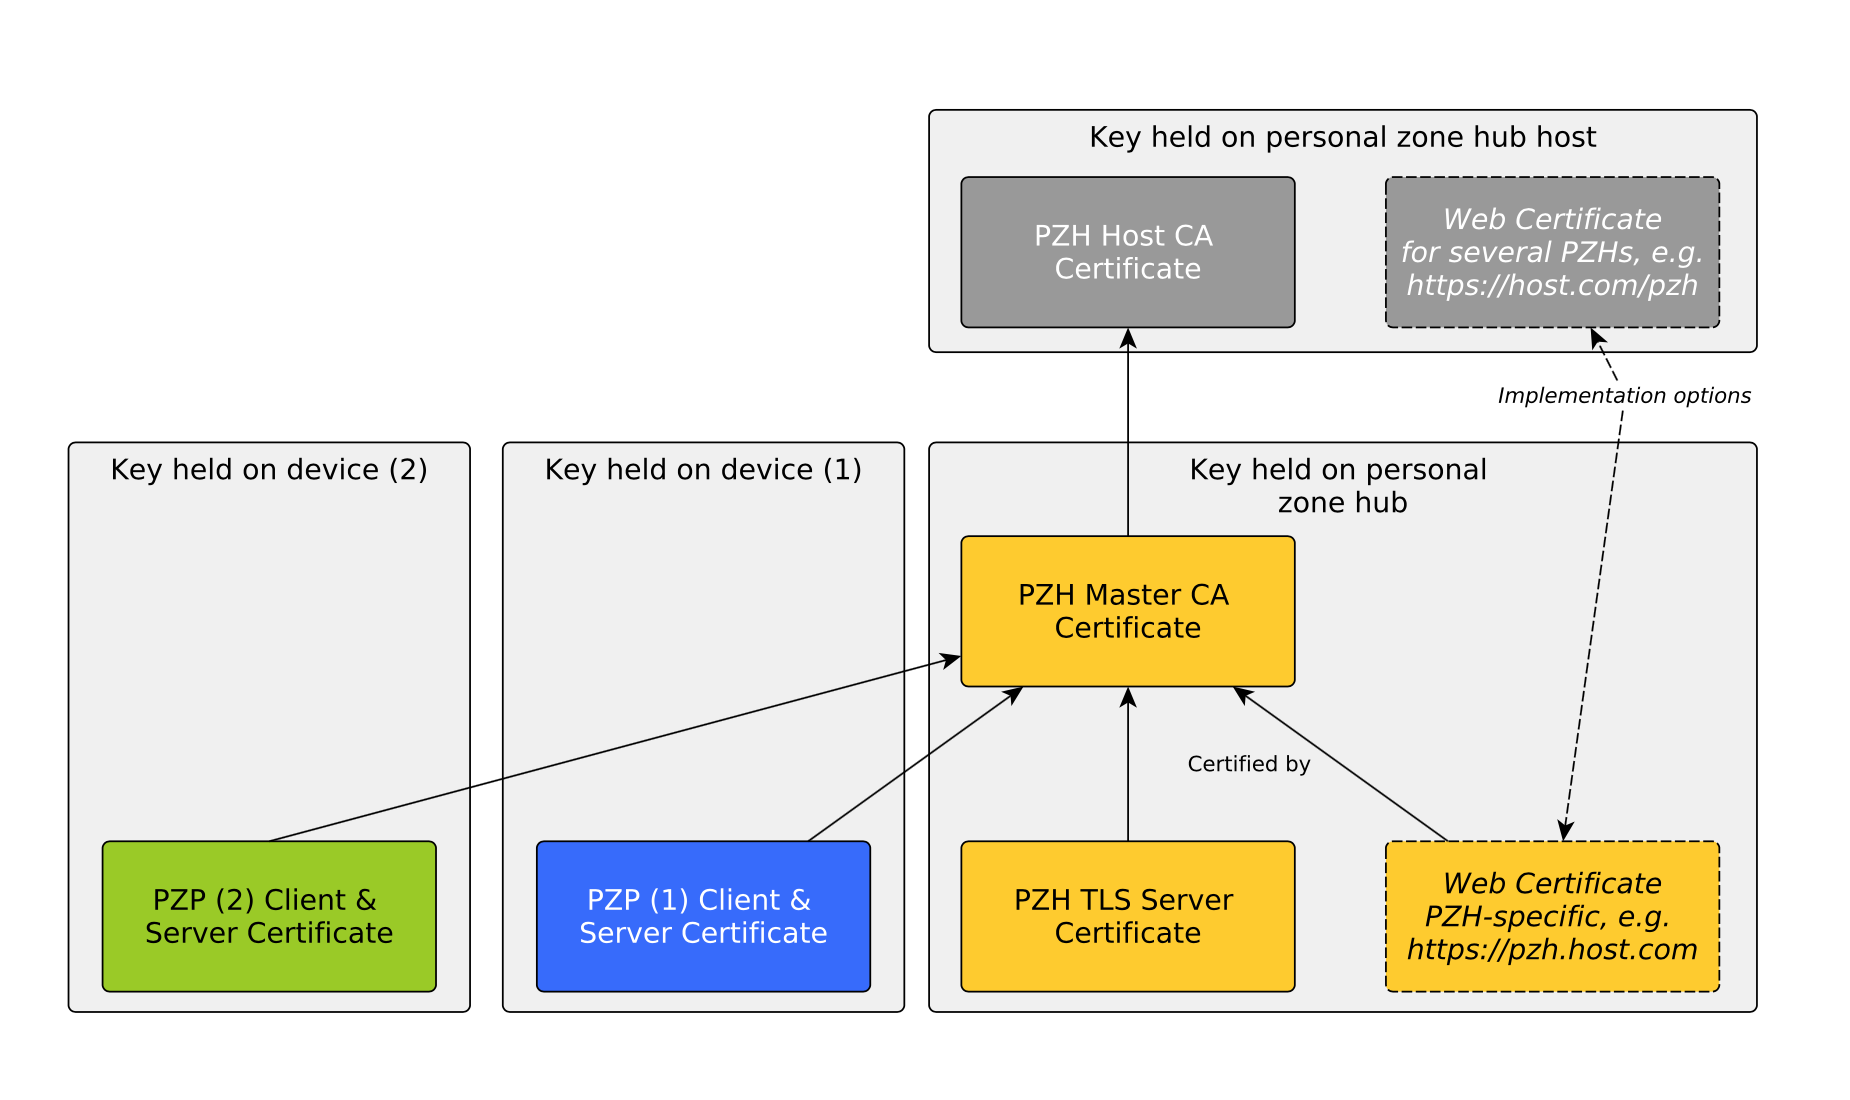
\includegraphics[width=\textwidth]{heir}
			\caption{Certificate heirarchy in \textit{webinos} \cite{Lyle2013}}
			\label{fig:heir}
		\end{figure*}
		An example of the certificate heirarchy is shown in Figure \ref{fig:heir}. The Personal zone hub acts as the certificate authority for the 					personal zones. The certificates are used to create mutually-authenticated TLS sessions. Users can host this hub on a home server if they 				wish.

	\item \textbf{User discovery} An existing personal identity is linked to the \textit{webinos} personal zone hub. The authors suggest using the 		WebFinger protocol\cite{Webfinger}.
	
	\item \textbf{Certificate exchange} \textit{webinos} requires that CA certificate exchange take place when two devices from differnet 					personal zones communicate for the first time. \textit{webinos} allows users to exchange certificates both when the devices are in close 				proximity and when they are far apaart (i.e. over the internet) and has separate specifications for both. When the devices are in close 						proximity, \textit{webinos} performs a ``peer to peer offline exchange''. When a user would like to access another user's API over the 					internet, \textit{webinos} performs an ``online exchange''. For the ``online exchange'' a user (say, Alice) can vists another user's (say, Bob's) 	PZH URL and make a request to access resources. \comment{add more details?}
	
	\item \textbf{Enrolment} Enrolment of a device has been kept relatively simple as well as user friendly. The user must install \textit{webinos} 		PZP onto their new device and then visits the PZH webpage, logs in and then simply adds a new device. The user is presented with a token such 	a QR code which they must enter into their new device. The specifics of the certificate exchange is completely hidden from the user.
	
	\item \textbf{Revocation of personal zone devices} Again, revocation of a lost or stolen device is acheived quite simply by visiting the hub 				website and clicking the revoke button for that the device. \textit{webinos} deals with revokation in the following manner: Each device (PZP) is 		made to maintain a Certificate Revocation List (CRL) and must synchronize this to the hub everytime it makes a new connection. The author's 		reason that this is sufficient protection against malicious attackers as it limits their window. It should be noted, however, that the author's also 		reason that in most cases, an 	average user's device would be stolen simply for the monetary value rather than an orchestrated malicious 				attack to steal the keys on it.
	
	\item \textbf{Access control and authentication} When a request is made the PZP will check whether the application, device \textit{and} user 		are are authorized to make that request. \textit{webinos} does not automatically associate a device with an individual user's identity except in 		certain cases where it is known that the device is user specific. For example, a user will not have to re-authenticate when a policy request is 			originating from their smartphone however, they will have to re-authenticate if the policy request is originating form their TV. This is a feature 		in particular, marks \textit{webinos} apart and makes it stand out. 
	
	\item \textbf{Key Storage} \textit{webinos} makes use of OS-provided mechanisms to securely store private keys. For example, the  						macOs Keychain app and the GNOME Keyring or some trusted platform-specific application. \comment{more info?}
	
	\item \textbf{Backup and Recovery} The authors have decided against any form of backup or recovery for \textit{webinos}. They reason that 		the user's OpenID account (or which ever onlin identity is used) will already have a password recovery feature in place. Also, lost of stolen 				devices may simply be revoked. If a key is compromised on an one device, that device can simply be revoked and re-added.

\end{enumerate}

\subsection{CONIKS}

\section{Threshold Cryptography}

The Threshold Cyptosystem approach to the multi-device problem has seen significant interest and development in the last few years. 

\subsection{Shatter}

\subsection{Blockchains and CoSi}

\section{Conclusions}

\comment{ device key also authenticates user. only webinos allows for multiple users on shared device because the device key only authenticates the device not the user}
